\chapter{Conclusion and Further Work}\label{cha:conclusion}
This report has presented and taken advantage of functional encryption schemes to define functional key exchange, which has been compared to standard group key exchange with the conflict between authentication and privacy being a central theme. It has been discussed how these schemes can be utilized and what limitations such a setup has.

\section{Conclusion}
This project has fulfilled the goals given in section \ref{sec:scope} of the introduction by :
\begin{itemize}
 \item Showing how functional encryption can be used to exchange keys securely, and applied the techniques of functional key exchange in a distributed chat room. Chapter \ref{chp:funckeyenc} introduced functional encryption and presented \gls{abe} in detail using implementations from the Charm toolbox. Two functional key exchange schemes was described in sections \ref{sec:abake} and \ref{sec:ibake}, before possible applications were discussed in section \ref{sec:apps}.
\item Proposing an attribute-based key exchange scheme using \gls{abe} as m\gls{kem} to exchange keys between multiple users, in chapter \ref{chp:designimpl}.
\item Implementing a system realizing and taking advantage of \gls{abake} to exchange keys, this in form of a chat room. The features of the system and models describing it are provided in sections \ref{sec:chat} and \ref{sec:models}. While the security requirements are discussed in section \ref{sec:concerns}. Finally the prototype is demonstrated in section \ref{sec:demo} with two users exchanging keys and computing a common session key which is used to encrypt and authenticate the communication.
\end{itemize}

With these results the project has shown that functional key exchange can be used in real systems where privacy is an important concern, and that implementing such systems is possible without too sever problems. 

\section{Further Work}
The extended system would include a separate \gls{kms} which the users would register with to obtain their key. The best solution would probably be to have a separate virtual or physical server doing each task; attribute and key management, storage and distribution of keying material, broadcasting of chat messages/cipher texts. Figure \ref{fig:improved} shows how the extended system would look on a high level. Other features like being able to create your own rooms and administrate these would also be logical. The prototype presented here will be a single room with a static policy.

\begin{figure}
\centering
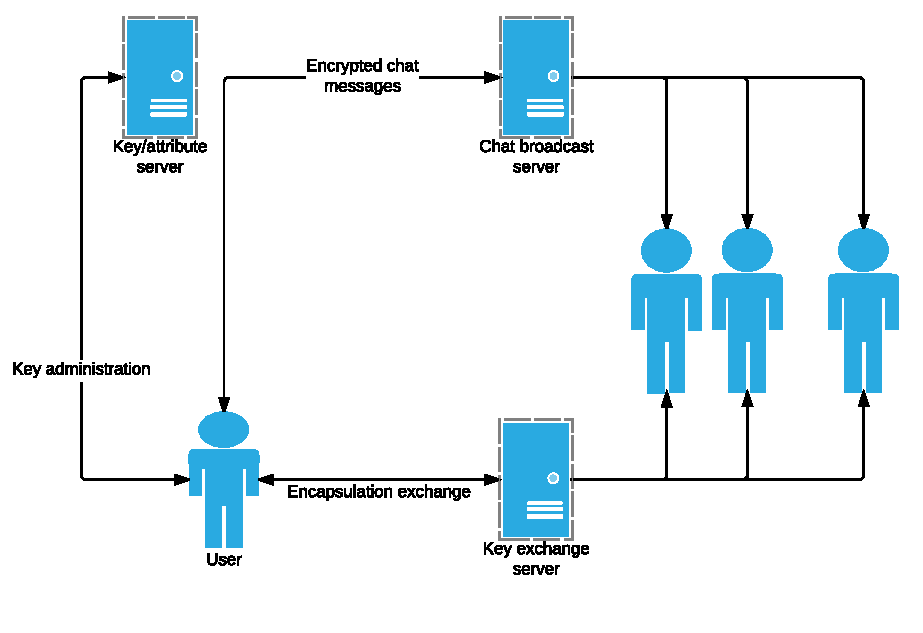
\includegraphics[trim=0cm 0cm 0cm 0cm, scale=0.8]{complete-system.pdf}
\caption{Improved system architecture}
\label{fig:improved}
\end{figure}

\par Another interesting extension to the system would be to remove the broadcast servers completely and apply a peer-to-peer setup, where the users distribute the encapsulations and the chat messages with the help of a broadcast server. The users would have to broadcast their encapsulations individually, the structure would look much like the one in group Diffie-Hellman as described in \ref{subsec:DH}. The users would need to have some way of knowing where to send their encapsulations. This could be solved by using multicast groups, which new users subscribe to, allowing them to receive new encapsulations, this would essentially be the same as the configuration used in this project. This setup would also require the users to negotiate the policy of the room without an intermediate server keeping track of this. To avoid pauses in the communication, the key exchange could be done in parallel while still using the old key, changing to the new one when finished. 

\par What is not clear is how this and similar systems behaves when the load of users increase, and lots of new keys have to be generated. This could be tested and acted upon, by setting up a testing environment and systematically test for different cases with users joining and leaving rapidly.

